% Se puede agregar el argumento 'twoside' a la par de letterpaper si se
% quiere imprimir dúplex, como libro
\documentclass[10pt, letterpaper]{report}
\usepackage[spanish,mexico]{babel}
\selectlanguage{spanish}
\usepackage[utf8]{inputenc}
\usepackage[T1]{fontenc}

\title{Plantilla para Trabajos de Graduación UVG}
\author{MSc. Miguel Zea}
\date{\today}

% Comandos definidos por el usuario en el archivo comandos_usuario.tex
%\input{paquetes_y_comandos_usuario}

% Información del estudiante en el archivo datos_estudiante.tex
% ================================================================================
% El estudiante debe llenar sus datos en esta sección para que la plantilla los 
% auto-importe y genere automáticamente las páginas de portada y de firmas 
% autorizadas.
% ================================================================================
% Datos del estudiante:
% --------------------------------------------------------------------------------
% Nombre completo
\def \nombreestudiante {Álvaro Roberto Sánchez Tórtola}
% Carné
\def \uvgcarne {13657}
% Facultad
\def \uvgfacultad {Ingeniería}
% Carrera
\def \uvgcarrera {Ingeniería en Ciencias de la Computación y Tecnologías de la Información}

% Datos del trabajo:
% --------------------------------------------------------------------------------
% Título completo
\def \titulotesis {Megaproyecto Detección Automatizada del Engaño (DAE): Módulo de Análisis Electroencefalográfico Empleando Máquina de Vectores de Soporte}
% Mes de entrega
\def \mesentrega {octubre }
% Año de entrega
\def \anoentrega {2018}
% Asesor
\def \nombreasesor {Ing. Tomás Gálvez Peña}

% Datos del tribunal examinador:
% --------------------------------------------------------------------------------
% Nombre del primer examinador
\def \nombreprimerex {MSc. Douglas Barrios}
% Nombre del segundo examinador
\def \nombresegundoex {Tribunal Examinador}
% Fecha de aprobación
\def \fechaaprobacion {-}

% Capítulos pre-definidos
% --------------------------------------------------------------------------------
% Comentar las líneas de las secciones que desean omitirse, por defecto se 
% se incluyen todas.
\def \CAPprefacio {Prefacio}
\def \CAPagradecimientos {Agradecimientos}
\def \CAPantecedentes {Antecedentes}
\def \CAPalcance {Alcance}
\def \CAPanexos {Anexos}
\def \CAPglosario {Glosario}
\def \CAPsimbolos {Listado de símbolos}

% Formato y estilo de la plantilla
% --------------------------------------------------------------------------------
% Portada: Puede cambiarse la imagen en la portada al cambiar el nombre del 
% archivo siguiente. NOTA: debe tener la suficiente resolución para cubrir el área
% designada
\def \imagenportada {plantilla/portadacit.jpg}
% Referencias: Puede des-comentar la siguiente línea para utilizar el formato de referencias APA
%\def \usarAPA {Usar formato APA}
% Párrafo: Puede comentar la siguiente línea si desea emplear un formato de 
% párrafo distinto al establecido por defecto
\def \parpordefecto {Formato de párrafo por defecto}
% Capítulos y secciones: Puede des-comentar la siguiente línea para establecer el 
% formato de los capítulos y secciones bajo el estándar original de UVG para
% trabajos de graduación. Este incluye: capítulos con numeración romana, secciones
% con letras mayúsculas, sub-secciones con números y sub-sub-secciones con letras
% minúsculas
%\def \capsecuvg {Formato UVG para capítulos y secciones}
% ================================================================================
% En este archivo se colocan opciones adicionales para modificar el formato de la
% plantilla, para emplearse en otros tipos de documentos que no sean trabajos de
% graduación. Si usted está trabajando su tesis, NO modifique este archivo
% ================================================================================
% Capítulos pre-definidos
% --------------------------------------------------------------------------------
% Comentar las líneas de las secciones que desean omitirse, por defecto se 
% se incluyen todas.
\def \CAPportada {Portada}
\def \CAPcaratula {Caratula}
\def \CAPfirmas {Hoja de firmas}
\def \CAPindice {Índice general}
\def \CAPfiguras {Listado de figuras}
\def \CAPcuadros {Listado de cuadros}
\def \CAPresumen {Resumen}
\def \CAPintroduccion {Introducción}
\def \CAPobjetivos {Objetivos}
\def \CAPjustificacion {Justificación}
\def \CAPmarcoteorico {Marco teórico}
\def \CAPconclusiones {Conclusiones}
\def \CAPrecomendaciones {Recomendaciones}
\def \CAPbibliografia {Bibliografía}

% ================================================================================
% DEFINICIÓN DE PAQUETES
% ================================================================================
\usepackage{xcolor}
\usepackage{amsfonts}
\usepackage{amsmath}
\usepackage{amssymb}
\usepackage{amsthm}
\usepackage{amsfonts}
\usepackage{mathtools}
\usepackage{graphicx}
\usepackage{xfrac}
\usepackage{float}
\usepackage{mathtools}
\usepackage[hypertexnames=false]{hyperref}
% \usepackage{bookmark}
\usepackage{subcaption}
\usepackage{babelbib}
\ifdefined\usarAPA 
	\usepackage{apacite} 
\fi
\usepackage[percent]{overpic}

\ifdefined\CAPglosario
	\usepackage[toc]{glossaries}
	\makeglossaries
    \newglossaryentry{latex}
{
    name=latex,
    description={Es un lenguaje de marcado adecuado especialmente para la creación de documentos científicos}
} 
 
\newglossaryentry{formula}
{
    name=fórmula,
    description={Una expresión matemática} 
}
\fi
\ifdefined\CAPsimbolos
	\usepackage[intoc, spanish]{nomencl}
	\makenomenclature
    \nomenclature{$c$}{Velocidad de la luz en el vacío}
\nomenclature{$h$}{Constante de Plank}
    \renewcommand{\nomname}{Lista de Símbolos}
\fi

% ================================================================================
% MÁRGENES Y FORMATO GENERALES
% ================================================================================
\usepackage[top=1in, left=1.5in, right=1in, bottom=1in]{geometry}
%Options: Sonny, Lenny, Glenn, Conny, Rejne, Bjarne, Bjornstrup
\usepackage[Sonny]{fncychap}
% ================================================================================
% DEFINICIONES DE LA PLANTILLA
% ================================================================================
\definecolor{uvg-green}{RGB}{17,71,52}
\newcommand{\defaultparformat}[1]{
	{\setlength{\parskip}{2ex}
    \input{#1}}
}
\ifdefined\capsecuvg
	\renewcommand\thechapter{\Roman{chapter}}
    \renewcommand\thesection{\Alph{section}}
	\renewcommand\thesubsection{\arabic{subsection}}
    \renewcommand\thesubsubsection{\alph{subsubection}}
\fi
% ================================================================================

% Comandos definidos por el usuario en el archivo comandos_usuario.tex
\input{paquetes_y_comandos_usuario}

% ================================================================================
% CUERPO DEL TRABAJO
% ================================================================================
\pagestyle{headings}
\begin{document}
% ================================================================================
% PORTADA
% ================================================================================
\ifdefined\CAPportada
% 	\cleardoublepage\phantomsection
%     \pdfbookmark{Portada}{toc}
	\newgeometry{left=3cm, bottom=0in, top=1in, right=3cm}
	\pagecolor{uvg-green}
	\thispagestyle{empty}

	\color{white}
	\noindent \hrulefill \par
	\vspace{0.1in}
	\noindent \Huge \titulotesis \par
	\noindent \hrulefill \par
	\noindent
	\LARGE \nombreestudiante

	\begin{figure}[b!]
    	%\makebox[\textwidth]{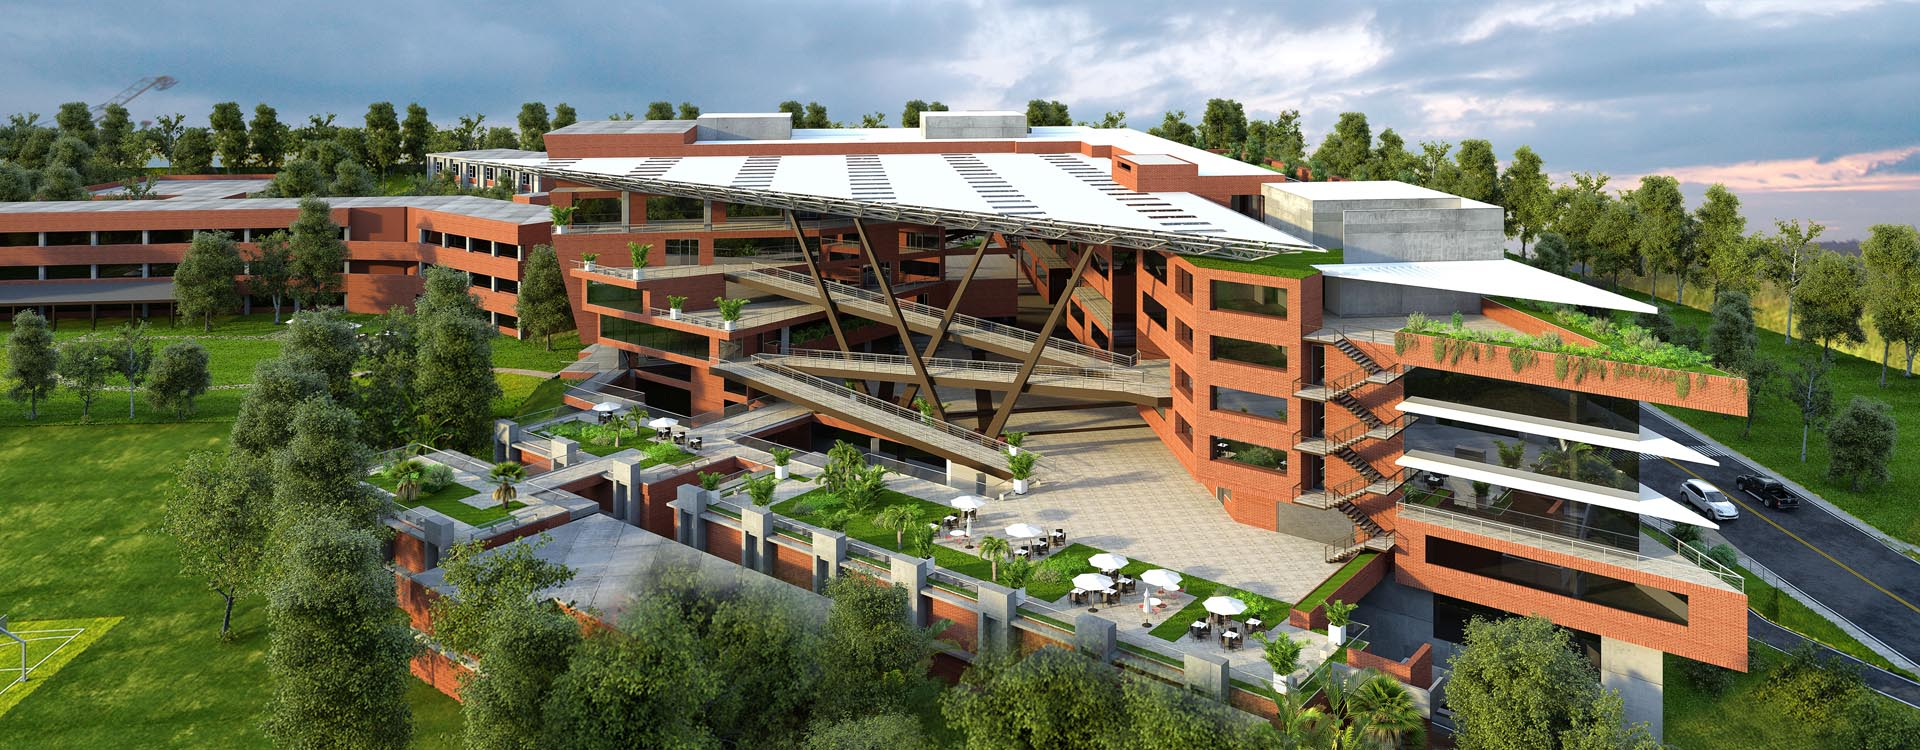
\includegraphics[height=13.25cm]{plantilla/portadacit.jpg}}
    	\makebox[\textwidth]{
    		\begin{overpic}[height=13.25cm]{\imagenportada}
     		\put(63,0){
\includegraphics[height=1.15in]{plantilla/fondologo_grande.png}}  
  			\put(64.5,2){
\includegraphics[height=0.55in]{plantilla/logoUVGblanco.eps}} 
        	\end{overpic}
    	}
    	%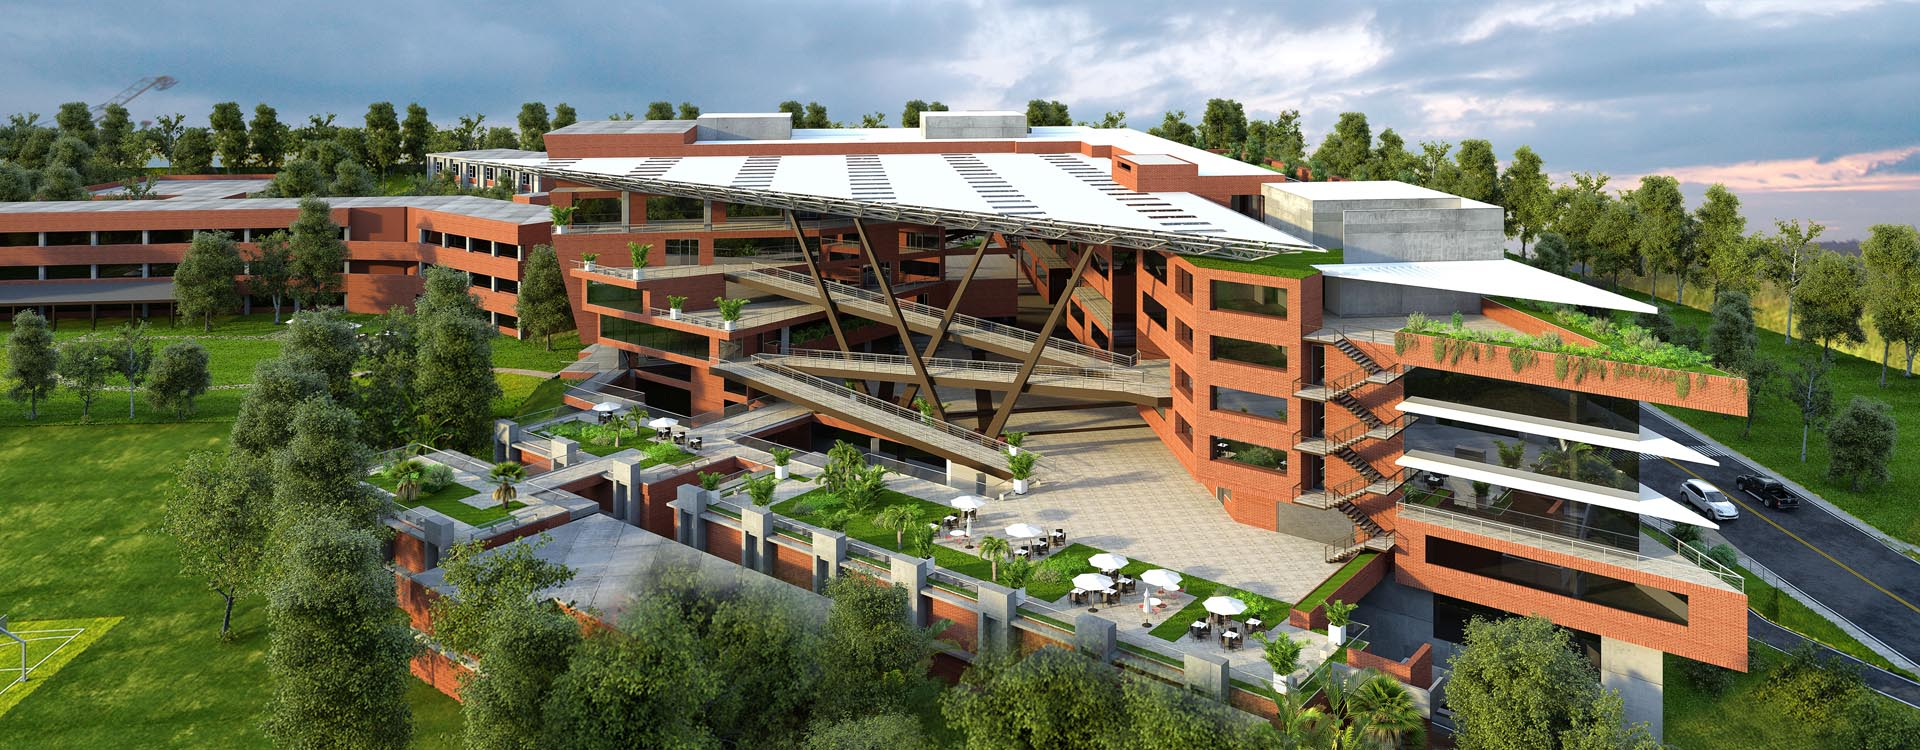
\includegraphics[height=13.25cm]{plantilla/portadacit.jpg}
	\end{figure}
	\restoregeometry
\fi

% ================================================================================
% PRIMERA PÁGINA
% ================================================================================
\ifdefined\CAPcaratula
	\newpage
%     \cleardoublepage\phantomsection
%     \pdfbookmark{Carátula}{toc}
	\pagecolor{white}
	\color{black}
	\setcounter{page}{1}
	\pagenumbering{roman}
	\thispagestyle{empty}
	\begin{center}
		\LARGE UNIVERSIDAD DEL VALLE DE GUATEMALA\\
		\LARGE Facultad de \uvgfacultad \\[0.75cm]
	\end{center}
	\begin{figure}[h]
		\begin{center}
		
\includegraphics[height=5.5 cm]{plantilla/escudoUVGnegro.eps}
		\vspace{0.5in}
		\end{center}
	\end{figure}
	\begin{center}
		\LARGE \textbf{\titulotesis} \\
		\vfill
		\vfill
		\Large Trabajo de graduación en modalidad de Megaproyecto presentado por \\
		\Large \nombreestudiante \\
		\Large Para optar al grado académico de Licenciado en \uvgcarrera \\
		\vfill
		\large Guatemala, \mesentrega del \anoentrega
	\end{center}
\fi

% ================================================================================
% HOJA DE FIRMAS
% ================================================================================
\ifdefined\CAPfirmas
	\newpage
	\thispagestyle{empty}
	\vspace*{0.5in}
	\large Vo.Bo.:\\[1cm]
	\begin{center}
		(f) \rule[1pt]{4 in}{1pt}\\
		\nombreasesor
	\end{center}
	\vspace{1in}

	Tribunal Examinador:\\[1cm]
	\begin{center}
		(f) \rule[1pt]{4 in}{1pt}\\
		\nombreasesor \\[1in]
		(f) \rule[1pt]{4 in}{1pt}\\
		\nombreprimerex \\[1in]
		(f) \rule[1pt]{4 in}{1pt}\\
		\nombresegundoex
	\end{center}
	\vspace{1in}

	Fecha de aprobación: Guatemala, \fechaaprobacion.
	\normalsize
\fi

% ================================================================================
% CONTENIDO DEL TRABAJO
% ================================================================================
% PREFACIO
% --------------------------------------------------------------------------------
\ifdefined\CAPprefacio
	\newpage
	\cleardoublepage\phantomsection
    \chapter*{Prefacio}
    \ifdefined\parpordefecto
    	\defaultparformat{prefacio}
    \else
    	En la actualidad, los procedimientos para la detección del engaño en el ámbito empresarial son muy limitados.  En la mayoría de las empresas, cuando se necesita realizar estas pruebas, se recurre al polígrafo. Sin embargo, el uso de este dispositivo no lanza un resultado muy preciso. La necesidad de obtener resultados más exactos nos llevan a buscar recursos en las neurociencias que nos permitan alcanzarlos.  El desarrollo de la inteligencia artificial en los últimos años ha generado nuevas alternativas para afrontar esta problemática. En este módulo se obtendrá información procedente del análisis electroencefalográfico aplicado a varios individuos; con el objetivo de detectar si los resultados de los mismos nos muestran cambios significativos que nos lleven a comprobar si los mismos, están mintiendo. Se utilizará algoritmos basados en Máquina de Vectores de Soporte no lineal para el procesamiento de los datos electroencefalográficos, provenientes del dispositivo \textit{Emotiv Epoc}. Como resultado, se obtendrán las características de estas señales que mejor puedan detectar el engaño, se producirá el código de un programa de detección de engaño, el porcentaje de efectividad del mismo y la interfaz de uso.
    \fi
    \addcontentsline{toc}{chapter}{Prefacio}
\fi

% AGRADECIMIENTOS
% --------------------------------------------------------------------------------
%\ifdefined\CAPagradecimientos
%	\newpage
%    \cleardoublepage\phantomsection
%	\chapter*{Agradecimientos}
%	\ifdefined\parpordefecto
%    	\defaultparformat{agradecimientos}
%    \else
%    	Class aptent taciti sociosqu ad litora torquent per conubia nostra, per inceptos himenaeos. Sed vulputate, metus vel efficitur fringilla, orci ex ultricies augue, sit amet rhoncus ex purus ut massa. Nam pharetra ipsum consequat est blandit, sed commodo nunc scelerisque. Maecenas ut suscipit libero. Sed vel euismod tellus.

Proin elit tellus, finibus et metus et, vestibulum ullamcorper est. Nulla viverra nisl id libero sodales, a porttitor est congue. Maecenas semper, felis ut rhoncus cursus, leo magna convallis ligula, at vehicula neque quam at ipsum. Integer commodo mattis eros sit amet tristique. Cras eu maximus arcu. Morbi condimentum dignissim enim non hendrerit. Sed molestie erat sit amet porttitor sagittis. Maecenas porttitor tincidunt erat, ac lacinia lacus sodales faucibus.

xxxxxxx

%    \fi 
%	\addcontentsline{toc}{chapter}{Agradecimientos}
%\fi

% ÍNDICE GENERAL
% --------------------------------------------------------------------------------
\ifdefined\CAPindice
	\newpage
    %\cleardoublepage\phantomsection
	\renewcommand{\contentsname}{Índice}
    \phantomsection
    \pdfbookmark{\contentsname}{toc}
	\tableofcontents
\fi

% LISTADO DE FIGURAS
% --------------------------------------------------------------------------------
\ifdefined\CAPfiguras
	\newpage
    \cleardoublepage\phantomsection
	\renewcommand{\listfigurename}{Lista de Figuras}
	\listoffigures
	\addcontentsline{toc}{chapter}{Lista de Figuras}
\fi

% LISTADO DE CUADROS
% --------------------------------------------------------------------------------
\ifdefined\CAPcuadros
	\newpage
    \cleardoublepage\phantomsection
	\renewcommand{\listtablename}{Lista de Cuadros}
	\listoftables
	\addcontentsline{toc}{chapter}{Lista de Cuadros}
\fi

% RESUMEN
% --------------------------------------------------------------------------------
\ifdefined\CAPresumen
	\newpage
    \cleardoublepage\phantomsection
	\chapter*{Resumen}
	\ifdefined\parpordefecto
		\defaultparformat{resumen}
	\else
		Existe insuficiente integración de las diferentes técnicas para la detección del engaño que le facilite al especialista la toma de decisiones. El uso de polígrafo para esta tarea suele ser la manera más recurrente. Sin embargo, este instrumento posee un bajo porcentaje de efectividad al momento de detectar el engaño (Wolpe, Foster, & Langleben, 2010). Nuevas técnicas que emplean inteligencia artificial para solucionar este tipo de problemas apenas están saliendo a la luz, y su uso puede brindar una valiosa alternativa para abordar este problema.  
	\fi
	\addcontentsline{toc}{chapter}{Resumen}
\fi

% INTRODUCCIÓN
% --------------------------------------------------------------------------------
\ifdefined\CAPintroduccion
	\newpage
	\pagenumbering{arabic}
	\setcounter{page}{1}
	\chapter{Introducción}
	\ifdefined\parpordefecto
		\defaultparformat{introduccion}
	\else
		Existe insuficiente integración de las diferentes técnicas para la detección del engaño que le facilite al especialista la toma de decisiones. El uso de polígrafo para esta tarea suele ser la manera más recurrente. Sin embargo, este instrumento posee un bajo porcentaje de efectividad al momento de detectar el engaño (Wolpe, Foster, & Langleben, 2010). Nuevas técnicas que emplean inteligencia artificial para solucionar este tipo de problemas apenas están saliendo a la luz, y su uso puede brindar una valiosa alternativa para abordar este problema.  
	\fi
\fi

% OBJETIVOS
% --------------------------------------------------------------------------------
\ifdefined\CAPobjetivos
	\newpage
	\chapter{Objetivos}
	\ifdefined\parpordefecto
		\defaultparformat{objetivos}
	\else
		\section{Objetivo General}
Elaborar una herramienta automatizada que combine diferentes técnicas de modo que apoyen al especialista en la detección del engaño.

\section{Objetivos Específicos}
\begin{itemize}
\item Clasificar los datos obtenidos por el dispositivo \textit{Emotiv Epoc} para ser usados por el algoritmo de detección del engaño. 
\item Evaluar la efectividad de detección del engaño del algoritmo basado en \textit{Máquina de Vectores de Soporte}.
\item Diseñar una interfaz de usuario para el uso general del algoritmo de detección del engaño. 
\end{itemize}
	\fi
\fi

% JUSTIFICACIÓN
% --------------------------------------------------------------------------------
\ifdefined\CAPjustificacion
	\newpage
	\chapter{Justificación}
	\ifdefined\parpordefecto
		\defaultparformat{justificacion}
	\else
		La necesidad de alternativas para la detección del engaño dentro del ámbito empresarial hace atractiva la idea de emplear inteligencia artificial. Los datos fisiológicos medidos por el polígrafo, por ejemplo, reflejan la actividad del sistema nervioso autónomo (SNA), por lo que reflejan no solo actividad inusual durante un engaño, sino también ansiedad en general, independientemente de la causa (Wolpe et al., 2010). El uso de análisis electroencefalográfico en los individuos de estudio es un método más directo, donde poco se ha explorado (Wolpe et al., 2010). Por lo que nuevos métodos de detección basados en esta metodología pueden ser de gran aporte, tanto para el ámbito empresarial, como para el campo de la inteligencia artificial en nuestro país.   
	\fi
\fi

% MARCO TEÓRICO
% --------------------------------------------------------------------------------
\ifdefined\CAPmarcoteorico
	\newpage
	\chapter{Marco Teórico}
	\ifdefined\parpordefecto
		\defaultparformat{marco_teorico}
	\else
		\section{La Naturaleza del Engaño}
La detección del engaño y la confirmación de la verdad con la poligrafía convencional planteó una serie de problemas técnicos y éticos (Wolpe et al., 2010).  El análisis de señales electromagnéticas del cerebro se ha postulado como una alternativa viable para la detección de la mentira en ámbitos legales y profesionales. Incluso algunos métodos se promueven como más efectivos que el polígrafo convencional. Sin embargo, estos métodos aun poseen limitaciones en cuanto a la falta de exploración de los mismos y a la poca estandarización que se tiene en su campo de estudio (Wolpe et al., 2010). 
\section{El Cerebro Humano y su Actividad}
En la actualidad, se ha eludido la relación entre la estructura del cerebro humano con funciones humanas. De igual manera, se elude la relación entre patrones de actividad neuronal con actividades del ser humano (Davatzikos et al., 2005). El análisis de patrones cuantitativos en el espacio-tiempo de la actividad cerebral conlleva a un análisis multivariable, poco explorado a principios de siglo por la limitación del procesamiento de datos de aquel entonces. El uso de algoritmos de Machine Learning para clasificar complejos patrones de activación cerebral se ha empezado a abordar en diversos estudios (Davatzikos et al., 2005). 
\section{Aprendizaje de Máquina}
Support Vector Machine (SVM) es un poderoso método de clasificación que encuentra la hiper-superficie que maximiza el margen entre dos distribuciones (Chih-Wei Hsu, Chih-Chung Chang, 2008), las respuestas verdaderas y no verdaderas en nuestro caso. El objetivo de un SVM es producir un modelo que predice los valores objetivo de un set de datos, a partir de únicamente los atributos del mismo set.  Formalmente, se describe como: dado un set de valores de la forma \gls{(x_i,y_i), i=1, …, l donde x_i∈R^n y y∈〖{1,-1}〗^l}, el SVM (Boser, Guyon, & Vapnik, 1992) requiere la solución al siguiente problema de optimización: 
\section{Máquina de Vectores de Soporte}
\subsection{Kernels Lineales y no Lineales}




	\fi
\fi

% ANTECEDENTES
% --------------------------------------------------------------------------------
\ifdefined\CAPantecedentes
	\newpage
	\chapter{Antecedentes}
	\ifdefined\parpordefecto
    	\defaultparformat{antecedentes}
    \else
    	Puede encontrarse un trabajo similar en {\color[white]{ \cite{Thai2012} \cite{Boser1992} \cite{Wolpe2010}  \cite{Chih-WeiHsuChih-ChungChang2008} \cite{Tzotsos2006} \cite{Davatzikos2005} \cite{Revell2004} \cite{EPOC2003} \cite{EMOTIV2014} \cite{Umale2016} \cite{Russell2010} \cite{Belmonte2007} \cite{Alpaydn2014} \cite{Aydemir2013} \cite{James1985} \cite{Vicianova2015} \cite{Ekman2009} }}
    \fi  
\fi

% ALCANCE
% --------------------------------------------------------------------------------
\ifdefined\CAPalcance
	\newpage
	\chapter{Alcance}
	\ifdefined\parpordefecto
    	\defaultparformat{alcance}
    \else
    	%Podemos usar \Gls{latex} para escribir de forma ordenada una \gls{formula} matemática. 
Este trabajo no estará ligado directamente con el módulo de análisis de micro expresiones ni el módulo de reconocimiento de voz. Además, este proyecto busca ser una prueba de concepto o profundización sobre análisis previamente realizados. Este módulo tampoco se enfoca en la generación del método para conducir al engaño en las pruebas a realizar. Se busca, específicamente, obtener un algoritmo de detección del engaño basado en \textit{Máquina de Vectores de Soporte}, un valor de efectividad de este, y el diseño de una interfaz para su uso.   
    \fi 
\fi

% CAPÍTULOS
% --------------------------------------------------------------------------------
\newpage
\ifdefined\parpordefecto
	\defaultparformat{capitulos}
\else
	%\chapter{Derivación de la dinámica del mecanismo}
%\section{Dinámica de cuerpos rígidos}
%\section{Restricciones}
%\subsection{Mecanismos de lazo cerrado}
%\subsubsection{Mecanismo de cuatro barras}
%\chapter{Control del sistema mecánico}
%\section{La ecuación del manipulador}
\fi

% CONCLUSIONES
% --------------------------------------------------------------------------------
\ifdefined\CAPconclusiones
	\newpage
	\chapter{Conclusiones}
	\ifdefined\parpordefecto
		\defaultparformat{conclusiones}
	\else
		Los datos clasificados permitieron identificar a las variables más significativas. Las variables descriptivas de mayor significancia fueron: edad, escolaridad, empleo y acompañamiento psicológico. Respecto a las variables electroencefalográficas, el canal F3 fue el más representativo. Sin embargo, ésta no fue mucho mayor que los canales AF3 y AF4. 

Los kernels empleados para Máquina de Vectores de Soporte fueron: Lineal, Polinomial y Gaussiano RBF. El mejor desempeño lo tuvo el modelo con kernel Gaussiano RBF. Este modelo tuvo un desempeño de precisión del cincuenta y ocho (58) por ciento para detectar el engaño. Sus mejores variables $\gamma$ y $C$ fueron $2^{-9.63}$ y $2^3$ respectivamente.

La interfaz de usuario para el manejo del sistema de detección del engaño por parte de estudiantes de la facultad de Psicología fue descrita como "\textit{sencilla y fácil de entender}". Sin embargo, no resultó ser "\textit{intuitiva}" al momento de utilizarse por primera vez.

De esta manera, se logró elaborar una herramienta automatizada para apoyar a la detección del engaño empleando Máquina de Vectores de Soporte con kernel Gaussiano RBF. Sin embargo, este método no alcanzó el mejor desempeño de precisión del engaño, por lo que es recomendado emplear un modelo como \textit{K Vecinos Cercanos}.
	\fi
\fi

% RECOMENDACIONES
% --------------------------------------------------------------------------------
\ifdefined\CAPrecomendaciones
	\newpage
	\chapter{Recomendaciones}
	\ifdefined\parpordefecto
		\defaultparformat{recomendaciones}
	\else
		En cuanto a la elección de características de medición para la detección del engaño, se recomienda experimentar y explorar otras características descriptivas que puedan brindar un perfil más específico de los sujetos de prueba. Características inusuales o que puedan segmentar de una mejor manera a la población objetivo, puede brindar un acercamiento distinto para la detección de sus emociones. Del mismo modo, escoger una población de estudio más amplia y general puede ayudar a representar de una mejor manera al ser humano como tal. Es decir, un mayor número de participantes y una mayor variabilidad en las características de estos puede ayudar a generalizar los elementos presentes en los seres humanos para la detección efectiva del engaño.

En cuanto a los modelos de predicción desarrollados, se recomienda utilizar el algoritmo \textit{K Vecinos Cercanos} para la predicción del engaño utilizando señales electroencefalográficas. Sin embargo, sería de mucho interés implementar combinaciones de algoritmos, como Máquina de Vectores de Soporte combinado con K Vecinos Cercanos, para obtener algoritmos más robustos y verificar si existe una mejora en la predicción del engaño de esta manera. Por otro lado, se recomienda realizar el procesamiento de los datos en un sistema operativo que permita a la librería \textit{TensorFlow} utilizar la tarjeta de vídeo externa para una mayor capacidad de procesamiento. Para eso, podría emplearse el sistema operativo \textit{Microsoft Windows} en conjunto con las tecnología \textit{CUDA de Nvidia}. 
	\fi
\fi

% BIBLIOGRAFÍA
% --------------------------------------------------------------------------------
\ifdefined\CAPbibliografia
	\newpage
    \cleardoublepage\phantomsection
	\ifdefined\usarAPA
		\bibliographystyle{apacite}
	\else
		\bibliographystyle{babplain}
	\fi
	\bibliography{bibliografia.bib}
	\addcontentsline{toc}{chapter}{Bibliografía}
\fi

% ANEXOS
% --------------------------------------------------------------------------------
\ifdefined\CAPanexos
	\newpage
    \cleardoublepage\phantomsection
%     \begin{center}
%     	\vspace*{\fill}
%     	\Huge Anexos
%     	\vspace*{\fill}
%     \end{center}
    \addcontentsline{toc}{chapter}{Anexos}
    \renewcommand{\chaptername}{Anexo}
    \setcounter{chapter}{0}
	\renewcommand{\thechapter}{\Alph{chapter}}
	\ifdefined\parpordefecto
    	\defaultparformat{anexos}
    \else
    	\chapter{Código Fuente}
El código desarrollado para este trabajo de graduación se puede encontrar en el siguiente repositorio público:

\underline{\textit{https://github.com/AlvaroSanchezTortola/SVMs-for-Lie-Detection}}

\textcolor{white}{ \cite{Thai2012} \cite{Boser1992} \cite{Wolpe2010}  \cite{Chih-WeiHsuChih-ChungChang2008} \cite{Tzotsos2006} \cite{Davatzikos2005} \cite{Revell2004} \cite{EPOC2003} \cite{EMOTIV2014} \cite{Umale2016} \cite{Russell2010} \cite{Belmonte2007} \cite{Alpaydn2014} \cite{Aydemir2013} \cite{James1985} \cite{Vicianova2015} \cite{Ekman2009} \cite{Tan2006} \cite{Irimia-Dieguez2015} \cite{Park2013} }
    \fi
\fi

% GLOSARIO
% --------------------------------------------------------------------------------
\ifdefined\CAPglosario
	\newpage
	\printglossary
\fi

% LISTADO DE SÍMBOLOS
% --------------------------------------------------------------------------------
\ifdefined\CAPsimbolos
	\newpage
    \cleardoublepage\phantomsection
    \printnomenclature
\fi

\end{document}